\documentclass[twoside]{article}
\usepackage{aistats/aistats2022}
% If your paper is accepted, change the options for the package
% aistats2022 as follows:
%\usepackage[accepted]{aistats2022}

% If you set papersize explicitly, activate the following three lines:
%\special{papersize = 8.5in, 11in}
%\setlength{\pdfpageheight}{11in}
%\setlength{\pdfpagewidth}{8.5in}

\let\oldsection\section
\renewcommand{\section}[1]{\oldsection{\texorpdfstring{\uppercase{#1}}{#1}}}

% If you use natbib package, activate the following three lines:
\usepackage[round]{natbib}
\renewcommand{\bibname}{References}
\renewcommand{\bibsection}{\subsubsection*{\bibname}}

\usepackage[utf8]{inputenc} % allow utf-8 input
\usepackage[T1]{fontenc}    % use 8-bit T1 fonts
\usepackage{hyperref}       % hyperlinks
\usepackage{url}            % simple URL typesetting
\usepackage{booktabs}       % professional-quality tables
\usepackage{microtype}      % microtypography
\usepackage{graphicx}
\graphicspath{{figs/}}
%\usepackage{subfigure}
\usepackage{subcaption}
\usepackage{hyperref}       % hyperlinks
\usepackage[dvipsnames]{xcolor}

\hypersetup{ % SLJ: my standard paper setup...
	pdftitle={MAP convergence},
	pdfkeywords={},
	pdfborder=0 0 0,
	pdfpagemode=UseNone,
	colorlinks=true,
	linkcolor=blue, %mydarkblue,
	citecolor=blue, %mydarkblue,
	filecolor=blue, %mydarkblue,
	urlcolor=blue, %mydarkblue,
	pdfview=FitH,
	pdfauthor={Anonymous},
}

\usepackage[capitalise]{cleveref}
\newcommand{\RLP}[1]{\textcolor{red}{RLP:#1}}
\newcommand{\fdk}[1]{\textcolor{Periwinkle}{fdk:#1}}
\newcommand{\TODO}[1]{\textcolor{cyan}{TODO #1}}

% my packages
\usepackage{math_commands}
% some custom math commands
\newtheorem{proposition}{Proposition}
\newcommand*{\expect}[2][]{\ensuremath{\mathbb{E}_{#1} \left[ #2 \right] }} % expectation operator
\newcommand{\cond}{\,\vert\,}
\newcommand{\logpart}{A}
\newcommand{\conj}{\logpart^*}
\newcommand{\bregman}{\cB_\logpart}
\newcommand{\bregmanconj}{\cB_{\logpart^*}}
\newcommand{\nat}{\theta}
\newcommand{\m}{m}
\newcommand{\meanp}{\m}
\newcommand{\decrement}{D}
\newcommand{\linear}{\ell} % linearization of a function
\newcommand{\lr}{\gamma} % learning rate, or step-size
\newcommand{\lin}[1]{\left\langle#1\right\rangle}

\newcommand{\MAPm}{\hat \m_n}
\newcommand{\MAPt}{\hat \nat_n}
\DeclareMathSymbol{\shortminus}{\mathbin}{AMSa}{"39}


\hypersetup{draft}

\begin{document}

% If your paper is accepted and the title of your paper is very long,
% the style will print as headings an error message. Use the following
% command to supply a shorter title of your paper so that it can be
% used as headings.
%
%\runningtitle{I use this title instead because the last one was very long}

% If your paper is accepted and the number of authors is large, the
% style will print as headings an error message. Use the following
% command to supply a shorter version of the authors names so that
% they can be used as headings (for example, use only the surnames)
%
%\runningauthor{Surname 1, Surname 2, Surname 3, ...., Surname n}

\twocolumn[

\aistatstitle{Convergence Rates for the MAP of an Exponential Family, and Stochastic Mirror Descent -- an Open Problem}


\aistatsauthor{R\'emi Le Priol \And Frederik Kunstner \And  Damien Scieur \And Simon Lacoste-Julien }

\aistatsaddress{ Mila \And  UBC \And SAIT SAIL \And Mila} 
]

\begin{abstract}
We consider the problem of upper bounding the expected sub-optimality of the maximum likelihood estimate (MLE), or a conjugate maximum a posteriori (MAP) for an exponential family. 
Surprisingly, we found no general solution to this problem in the literature. 
In particular, current theories do not hold for a Gaussian, or in the very interesting few samples regime.
After exhibiting various facets of the problem, we show the MAP can be interpreted as the result of Stochastic Mirror Descent (SMD), 
yet it falls out of scope for modern analysis.
We believe solving this very fundamental problem may bring progress to both the statistics and optimization communities.
\end{abstract}

%In particular, no rates hold in the few samples regime  -- e.g. after seeing 5 samples from a gaussian, we do not know how many bits away from the true distribution we should expect our model to be.
%No rates hold either when the loss is ill-behaved : infinite domain, not smooth, not self-concordant


\section{Motivation}

We kind of know how to do optimization 
on smooth, strongly convex functions 
when there is some bound on the stochasticity,
for example in the form of a bounded variance, 
say for the problem 
\begin{equation}
\min_\theta f(\theta) 
\end{equation}
with access to stochastic gradients 
$g(\theta)$ such that 
\begin{equation}
	\expect{\norm{g(\theta) - \nabla f(\theta)}^2} \leq \sigma^2.
\end{equation}
Estimating the mean of Gaussian noise is a special case of this problem class, using 
$f(\theta) = \frac{1}{2}\norm{\theta - \mu}^2$ and $g(\theta) \sim \cN(- \mu, \sigma^2)$.
SGD with a decreasing step-size coincides with the maximum likelihood estimate (MLE), 
and attains the $1/t$ convergence rate.

But our understanding of stochastic optimization lacks in other domains. 
A generalization of the above problem, at the intersection of optimization and statistics, 
is the problem of minimizing 
\begin{equation}
	f(\theta) = \expect[x \sim p(x\cond\theta_*)]{-\log p(x\cond\theta)},
\end{equation}
When $p(x\cond\theta)$ is an exponential family distribution,
$-\log p(x\cond\theta) = A(\theta) - \lin{t(x), \theta}$ (omitting the reference distribution).
Here, $A$ is the log-partition function, a Legendre function that we assume can be minimized in closed form.
The Gaussian example is the special case $A(\theta) = \frac{1}{2}\norm{\theta}^2$.

There are algorithms for this setting, for example the MLE -- the (online) maximum likelihood after seeing $t$ samples -- or adding regularization, the MAP -- the maximum a posteriori.
As we show, the MAP can be interpreted as online mirror descent with decreasing step-sizes.
Despite recent advances in this field, our convergence rates are still lacking; they are either asymptotic, cover only special cases or require having seen many ($n \gg d$) samples.

We do not have a solution. The goal of this paper
is to bring this issue to the attention of the community working at the intersection of machine learning, optimization and statistics,
in the hope that we can make progress on this question;
Can we build algorithms for stochastic estimation 
when the objective function is not (close to) quadratic
and the noise is not Gaussian?

We are aware that \emph{a} solution to this problem would be the maximum likelihood estimate for which there is a wealth of asymptotic and large sample results \citep{van2000asymptotic,ostrovskii2021finite}. %TODO complete 
However, none of the theory we found could address for instance the case of a Gaussian with unknown mean and variance $\cN(\mu,\sigma^2)$, hence our contributions. 
%TODO kind of redundant "problem - question - problem" paragraphs, not disentangling stats and optim. To improve

\paragraph{Contributions}
\begin{itemize}
	\item We provide insights on different facets of this problem : quadratic approximations ; bias variance decomposition; and a detailed analysis of the Gaussian variance estimation problem.
	\item We show the connections between the optimization and statistical estimation view of the problem and discuss where current theories fail to fully capture the problem.
\end{itemize}

The statistics and optimization perspective are so tightly linked in this problem, that we believe progress from one field would help the other one. 
Progress from statistics could bring forward research in non-euclidean optimization, or the optimization of barrier losses, for instance helping in the development of accelerated methods.
On the other hand, optimization can become  a more versatile and general tool for statisticians. % handwavy and shady af.


% Then; 
% - description of the setting
% - statistical solutions (asymptotic, l1 or l2 error)
% - optimization solutions (online+bounded gradient, self-concordance, more recent relative smoothness results)
% - potential application of ideas that would solve this, beyond this problem (acceleration, causality?)
% - conclusion?


\section{Technical background}

Exponential Families are to statistics what linear models are to regression.
Many classical model are exponential families, and their convexity and modeling flexibility make them one of the most widely used statistical models. 
Here we review some of their properties. 
We point the reader towards \citet[Chapter 3]{wainwright2008graphical} for a full review.
The exponential family for data $X\in \cX$ with natural (or primal) parameter $\nat$  is specified by a sufficient statistic $T: \cX \rightarrow \real^d$ and a density with respect to a base measure $\nu(dx)$
\begin{equation}
	 p(X|\nat) = \exp( \nat^\top T(X) - \logpart(\nat)) \; ,
\end{equation}
Here $\logpart$ is the log-partition function -- i.e. the normalization term
\begin{align}
    \logpart(\nat) = \log \int e^{\nat^\top T(x)} \nu(dx) \; .
\end{align}
When explicit, we will write the random variable $T = T(X)$ for lightness.
For convenience, we focus on steep exponential families with $\logpart$ a convex function of Legendre type.
In particular, the set $\nat \in \Theta$ such that $\logpart(\nat) < \infty$ is open and convex.
This simple model encompasses both categorical distributions : $\cX = \{1, \dots, k\}, \nu$ uniform and $T(X)$  the one-hot encoding, and multivariate normal distributions $\cX=\real, \nu$ Lebesgues and $T(X)=(X, X^2)$. 

% TODO sort out relationships between : steep family, minimal statistics and Legendre type. What implies what ?

\paragraph{Duality}
The logpartition function $\logpart$ verifies the two following identities
\begin{align}
    \nabla\logpart(\nat) &=  \expect[p(T|\nat)]{T} =: \meanp \\
    \nabla^2 \logpart(\nat) &= \Cov_\nat[T] \geq 0
\end{align}
where $\meanp$ is called the mean (or dual) parameter.
From now on, we assume that the sufficient statistic $T$ is minimal 
-- e.g. its covariance is definite positive for all $\nat$ -- 
then the log-partition function $\logpart$ is strictly convex and its gradient $\nabla \logpart$ is a bijection between natural parameters $\nat$ and mean parameters $\m$.
$\meanp$ lives in the open convex set $\cM$ equal to the relative interior of the convex hull of $T(\cX)$.
We will write interchangeably $\m$ or  $\nat$ depending on the context, being aware that both represent the same distribution.
At this point it is useful to introduce the convex conjugate (a.k.a. Fenchel-Legendre transform) of the logpartition function
\begin{align}
	\conj(\m) = \langle \m, \nat \rangle - \logpart(\nat) \; .
\end{align}
which matches the common notion of \textit{entropy} in information theory.
The entropy is eating mean parameters, and its gradient is mapping back to natural parameters $\nabla\conj \circ \nabla\logpart(\nat) = \nat$ (cf Fig.~\ref{fig:duality}).

\begin{figure}[ht]
	\centering
	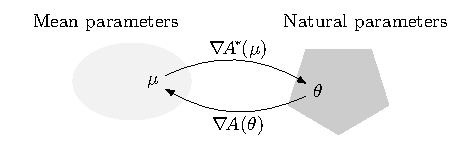
\includegraphics{duality}
	\caption{The gradient of the log-partition function and its dual, $(\nabla \logpart, \nabla \conj)$, form a bijection between natural and mean parameters $\nat, \meanp$. Figure copied from \citet{kunstner2020homeomorphic}. % TODO make an original one.
	}
	\label{fig:duality}
\end{figure}

\paragraph{Bregman Divergences}
A very useful object to keep in mind is the Bregman divergence induced by $\logpart$ between two parameters $\nat$ and $\nat_0$
\begin{align}
    \bregman (\nat ; \nat_0)
    & = \logpart(\nat) - \logpart(\nat_0) 
    - \langle \nabla \logpart(\nat_0)  , \nat - \nat_0 \rangle
\end{align}
with $\nabla \logpart(\nat_0) = \expect[\nat_0]{T(X)} =: \meanp_0$ the mean parameter associated to $\nat_0$. 
It is a non-symmetric measure of distance between parameters.
It is equal to the divergence of its convex conjugate with switched arguments
\begin{align}
	\bregman (\nat ; \nat_0)
    = \bregmanconj ( \meanp_0 ; \meanp) \; .
\end{align}

\paragraph{Conjugate Prior}
One conjugate prior \citep{agarwal2010geometric} for $p(X|\nat)$ is
\begin{align}
    p(\nat) 
    &\propto \exp( - n_0 \bregman(\nat ; \nat_0) ) \\
    &\propto \exp(n_0 \m_0^\top \nat - n_0 \logpart(\nat))
\end{align}
where $n_0$ and $\nat_0$ are (hyper)parameters of the prior.
This is the formula for the exponential family with sufficient statistics $(\nat ,\logpart(\nat))$ and with natural parameter $(n_0 \m_0, -n_0)$.
Intuitively, $n_0$ is a number of fictive data points observed from a distribution with parameter $\nat_0$.

\paragraph{Maximum A Posteriori (MAP).}
Using Bayes rule, the posterior of $\nat$ given a dataset $\mD_n =(X_1,\dots,X_n)$ is
\begin{align}
	p(\nat \cond \mD_n)
	%\propto p(\mD|\nat)p(\nat) 
    \propto \exp(- (n_0+n) \bregman(\nat; \MAPt))
    \label{eq:joint_likelihood}
\end{align}
reaching its maximum in $\MAPt$, the MAP estimate verifying the first order optimality conditions
\begin{align}
    \nabla \logpart(\MAPt) = \MAPm
    = \frac{n_0 \meanp_0 + \sum_{i=1}^n T_i}{n_0+n} \; .
\end{align}
where $T_i=T(X_i)$.
When $n_0=0$ -- eg we observed zero samples from the prior -- we recover the Maximum Likelihood Estimate (MLE)
\begin{align}
	\hat \m_n^\text{MLE} = \frac{\sum_{i=1}^n T_i}{n}
\end{align}
This last equation is known as moment matching.
The MLE and MAP estimates are statistics of the dataset $\mD_n$. 
Given a random dataset, we wish to bound their deviation from the optimum $\nat^*$ or $\meanp^*$.


\section{Open Problem}

Let $\nat^* := \argmin \expect[X\sim\cD]{-\log p(X|\nat)}$, where $\cD$ is any distribution such that $\E[T] = \meanp^* \in \cM$.
Then the suboptimality on the population log-likelihood is exactly the KL between our current model and the true distribution
\begin{multline}
    \expect[X\sim \cD]{-\log p(X|\nat) + \log p(X|\nat^*) } \\
	= \KL( p(.|\nat^*) ; p(.|\nat)) \; .
\end{multline}
Note that $\cD$ does not have to be part of the exponential family.
For the exponential family, the KL is equal to the Bregman divergence induced by the log-partition function, or alternatively by the entropy, being careful with the order of the arguments 
\begin{align}
\boxed{
	\KL( p(.|\nat^*) ; p(.|\nat))
    = \bregman (\nat ; \nat^*)
    = \bregmanconj ( \meanp^* ; \meanp)
}
\end{align}

Typical works on parameter estimation bound the deviation with norms -- e.g. bounding $\expect[p(x\cond\theta_*)]{\norm{\theta-\theta_*}^p}$ for some norm and some power. \TODO{cite} 
Or more generally, they  use distances rather than divergences as they are symmetric and usually behave smoothly. \TODO{cite} 
A contrario the KL is not smooth, and it can be infinite in misspecified settings.
But as the MLE is the minimizer of the log-likelihood, we wish to bound the sub-optimality.

Our question is: how does the KL behave when $\nat$ is the maximum-likelihood or the MAP estimate ? Can we get upper-bounds on the following quantities ?
\begin{align}
	\label{eq:bregmanMLE}
	\expect[\mD]{\bregmanconj \left (\E [T] ;  \inv{n}  \smallsum_i T_i \right )} \\
	\label{eq:bregmanMAP}
	\expect[\mD]{\bregmanconj \left (\E [T] ; \frac{n_0 \m_0 + \smallsum_i T_i}{n_0+n} \right )} 
\end{align}
where the outer expectation is on the dataset $\mD = \{X_1, \dots, X_n \}$ sampled i.i.d from $\cD$.
More explicitly, can we write an upper bound that does not involve an expectation over the dataset -- e.g. where the stochasticity is removed.


\paragraph{Remark.}
This could be seen as a concentration inequality, expressed with a Bregman divergence instead of a norm.
However there is a connection between the random variable $T(X)$ and the metric $\logpart$. 
Indeed expressions~\eqref{eq:bregmanMLE} or~\eqref{eq:bregmanMAP} can be infinite for another choice of random variable. 
For instance, if we plug in $\conj(\m)= -\log(\m)$, which defines a divergence on positive numbers, and $T(X) \sim \cN(0,1)$ which can be negative.

\paragraph{Remark 2.}
The expectation of the MLE may be infinite, for instance with $\cN(0,\sigma^2)$ and $n\leq 2$. Instead of taking the expectation,  we might want to bound this quantity in high probability, without resorting to Markov inequality, but that is a difficult endeavor.

\section{Insights}

\subsection{MAP as Stochastic Mirror Descent}
\label{ssec:MAP=SMD}
The posterior~\eqref{eq:joint_likelihood} can always be written iteratively $p(\nat | \mD_n) \propto p(X_n | \nat) p(\nat | \mD_{n-1})$, so that the MAP verifies
\begin{align*}
	\hat \nat_{n}
	= \argmin_\nat - \log p(X_{n} | \nat) + (n_0 + n -1) \bregman(\nat; \hat \nat_{n-1})
    %\label{eq:SBPP}
\end{align*}
which is the update of a Stochastic Bregman Proximal Point update with step-size $\inv{n_0 + n - 1}$. Expanding $p(X_{n} | \nat)$ and  playing with the Bregman we get
\begin{align}
		\hat \nat_{n}
	= \argmin_\nat g_{n}^\top \nat + (n_0 + n) \bregman(\nat; \hat \nat_{n-1})
    \label{eq:SMD}
\end{align}
where $g_{n} := \nabla\logpart(\hat \nat_{n-1}) - T(X_n) = \hat \m_{n-1} - T_n$ is the gradient of $-\log p(X_{n} | \nat)$ evaluated at $\hat \nat_{n-1}$. 
We recognize the update of Stochastic Mirror Descent (a.k.a. Stochastic Bregman Gradient) with step-size $\lr_n = \inv{n_0 + n}$ -- a stochastic gradient step in the dual $\hat \m_n = \hat \m_{n-1} - \lr_n g_n$.
This parallel means it would be possible to obtain a finite convergence rate for the  MAP from an analysis of these algorithms. 
We give a special focus on this approach in Section~\ref{sec:optimization}.


\subsection{Asymptote}
As a reference point for any finite convergence rate, it is interesting to know the asymptotic behavior of these quantities as $n \rightarrow +\infty$.
Asymptotic results typically show that natural parameters $\nat$ asymptotically normal ; reaching the Cramer-Rao lower bound \citep[for instance Ch4.2]{van2000asymptotic}.
Here the MAP is more simply expressed with mean parameters $\meanp$.
We get the asymptote by approximating the Bregman divergence using a second order Taylor expansion
\begin{align}
    \bregmanconj(\m^* ; \m) 
    &=\half  \norm{\m^* - \m}^2_{\nabla^2\conj(\m^*)}
    + O(\norm{\m - \m^*}^3)
\end{align}
where the Mahalanobis norm  $\| x \|_\mM^2 = x^\top \mM x$  is induced by the hessian of the entropy -- the inverse \textit{Fisher information matrix} -- at the optimum, 
\begin{align}
    \mF^*
    :=\nabla^2\conj(\m^*) 
    = \nabla^2\logpart(\nat^*)^{-1} 
    = \Cov_{\nat^*}[T(X)]^{-1}  \; .
\end{align}
From there, it is possible to show an asymptotic rate for the MLE and the MAP
\begin{align}
\label{eq:MAP_asymptote}
	\E \bregmanconj \left (\E [T(X)] ; \hat \meanp_n^\text{MLE/MAP} \right ) 
	= \frac{d}{2n} + O(n^{- \frac{3}{2}}) \; .
\end{align}
Both MLE and MAP have the same asymptote, as the contribution of the prior $n_0 \meanp_0$ gets negligible compared to the data for large $n$.
This asymptote is also independent of the optimum $\meanp^*$.

\subsection{Quadratic Case}
As another reference point, let us consider the case $\logpart(\nat) = \half \norm{\nat}_2^2$.
For instance, this is the log-partition of a Gaussian with variance $1$ and unknown mean ($\cX=\real, \nu(dx) = \exp(\half[-x^2])dx, T(X)=X$).
Then $\conj(\meanp) = \half \norm{\meanp}_2^2$ as well, and both Bregman divergences are squared $\ell^2$ distances
\begin{align}
	\bregmanconj(\meanp^* ; \meanp) = \half \norm{\meanp^* -  \meanp }_2^2  \; .
\end{align}
Thanks to the independence of samples we can break down the MLE into individual point's contributions
\begin{align}
	\expect{\half \norm{\m^* -  \inv{n}  \smallsum_i T_i}_2^2} 
	=\frac{\Var(T)}{2n} 
\end{align}
Adding a reference mean $\m_0$ to get the MAP yields
\begin{align}
	\expect{\bregmanconj(\meanp^*; \MAPm)}
	&= \frac{n \Var(T) +  n_0^2 \norm{\m^* -  \m_0}^2}{(n+n_0)^2}
	%\\ &= O\left(\frac{\Var(T)}{n} \right) + O\left(\frac{\norm{\m^* -  \m_0}^2}{n^2} \right)
	\label{eq:MAP_quadratic}
\end{align}
so we have a variance term in $O(n^{-1})$ and a bias term decreasing as $O(n^{-2})$. We would like to get a similar result for arbitrary exponential families.
If we make restrictive assumptions on the log-partition function, we can relate $\bregmanconj$ to a norm or a quadratic.

{\bf If $\conj$ is $L$-Lipschitz} (e.g. $\logpart$ is defined within the $\ell^2$-ball of radius $L$), then
\begin{align}
    \bregmanconj(\m^* ; \m) 
    &\leq L \norm{\m^* - \m} + \norm{\nat} \norm{\m^* - \m} \\
    &\leq 2L \norm{\m^* - \m}
\end{align}
so $\bregmanconj$ is $2L$-Lipschitz, and we get a $O(\inv{\sqrt{n}})$ rate.

{\bf If $\conj$ is $L$-smooth} (e.g. $\logpart$ is $\frac{1}{L}$-strongly convex), then
\begin{align}
    \bregmanconj(\m^* ; \m) 
    \leq \frac{L}{2} \norm{\m^* - \m}^2
\end{align}
so $\bregmanconj$ is upper bounded by a quadratic, and we get~\eqref{eq:MAP_quadratic} as an upper bound.

\subsection{Locally Quadratic Case}
All Bregman divergences are locally quadratic. 
Under some assumptions, we can quantify  when this quadratic behavior  kicks in.
For instance {\bf when $\conj$ is self-concordant} \citep[Ch.4.1]{nesterov2003introductory}. 
This is true when $T$ is 1-dimensional and $\logpart$ is self-concordant 
-- e.g. exponential distribution, 
Gaussian and Laplace distributions with known mean,
Pareto distribution with known minimum value, 
Weibull distribution with known shape k
-- or when $T$ lives in a compact \citep{bubeck2015entropic}. Then the bound
\begin{align}
	 \bregmanconj(\m^*,\m) \leq \norm{\m^*-\m}_{\mF^*}^2
\end{align}
holds whenever $\norm{\m^*-\m}_{\mF^*} < 0.21$. 
Similarly, \citet{kakade2010learning} assumes a bound on all higher order moments at $\nat^*$ to quantify when $\logpart$ starts behaving quadratically, but their rate does not directly apply to $\conj$ and $\m$.

\TODO{Reference \citet{ostrovskii2021finite}.} ( as well as 
\citet{anastasiou2017bounds},
\citet{marteauferey2019beyond})

All these works give \textit{large sample} results -- results that hold only for $n\geq N$ for some constant $N$ -- but none of them  apply to small $n$.

\subsection{Bias-Variance Decomposition}
In both examples (add link), the upper bound takes the form $O(\inv{n}) + O(\frac{\text{bias}}{n^2})$, reminding us of the bias-variance decomposition. In fact, it is possible to write such a decomposition for any Bregman divergence
Let $\tilde \theta_n := \expect{\hat \theta_n}$ be the expectation of the MAP in primal space, and $\tilde \m_n = \nabla \logpart(\tilde \theta_n )$ be the corresponding mean parameter.
As described by \citet[Theorem 0.1]{pfau2013generalized}, the  expected Bregman decomposes like
\begin{align}
	\expect{\bregmanconj(\m^* ; \hat \m_n)} 
	&= {\bregmanconj(\m^* ; \tilde \m_n)}
	+ {\expect{\bregmanconj(\tilde \m_n ; \MAPm)}}
	\label{eq:primal_pivot}
\end{align}

\textbf{Remark:} In this decomposition, the primal expectation $\expect{\hat \theta_n}$ is taking the role of pivot / reference point. An estimator will be unbiased if its primal expectation is non-zero. 
This is not true for the MLE. In fact for the gaussian variance MLE, the bias decreases like ${\bregmanconj(\m^* ; \tilde \m_n)} \leq \frac{2}{n(n-2)}$.
A contrario, the MLE is unbiased wrt the dual parameter, but the decomposition there is not clean.

\paragraph{Illustrations.}
We show these decompositions for $\cN(0,\sigma^2)$ in Figure~\ref{fig:variance_decomposition} and  $\cN(\mu, \sigma^2)$ in Figure~\ref{fig:gaussian_decomposition}.
In particular for $\cN(\mu, \sigma^2)$, we illustrate the characters featured in these decompositions $\hat \m_n^\text{MLE},\hat \m_n^\text{MAP},\m_n,\tilde \m_n, \m^*$ and $\m_0$ (and corresponding primal parameters)  in Figure~\ref{fig:bias-variance-numerical}. \RLP{Tune figures.}


\begin{figure*}[ht]
	\centering
	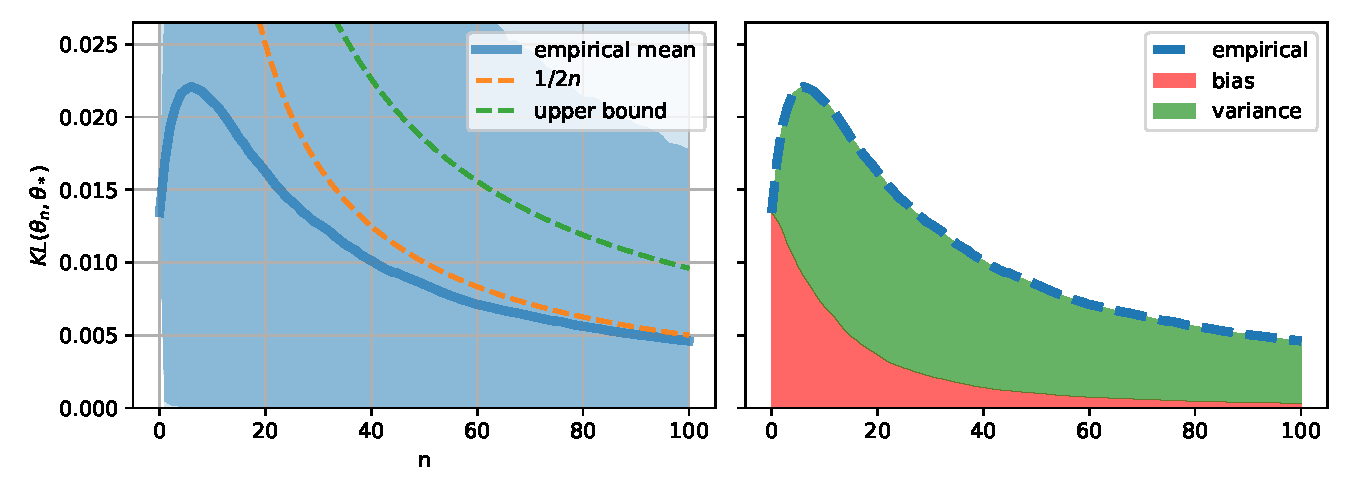
\includegraphics[width=\textwidth]{{figs/biasvariance/new_linear_ratio=0.8_n0=10}.pdf}
	\caption{
	\textbf{Gaussian variance $\cN(0,\sigma^2)$ example. Left:} training curves and analytic upper bound. 
	\textbf{Center:} bias-mixed-variance decomposition, using the arithmetic mean.
	\textbf{Right:} bias-variance decomposition, using the harmonic mean.
	}
	\label{fig:variance_decomposition}
\end{figure*}

\begin{figure*}[ht]
	\centering
	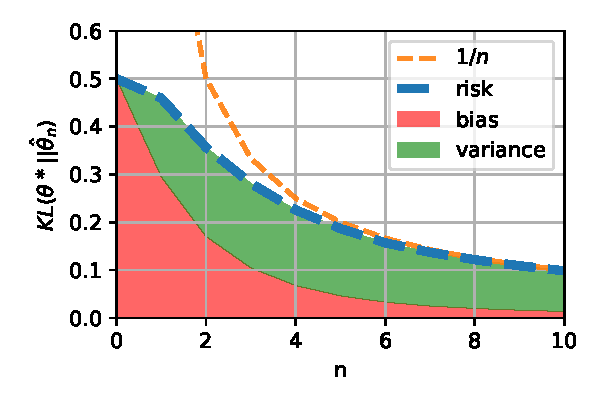
\includegraphics[width=\textwidth]{{figs/gaussians/new_linear_n0=1}.pdf}
	\caption{
	\textbf{Full gaussian} $\cN(m, \sigma^2)$ with $\meanp^*=(0, 1), \meanp_0 = (1,2)$ and $n_0=1$. \textbf{Left:} training curves (5,95) percentiles, average and asymptote. 
	\textbf{Right:} bias-variance decomposition.
	}
	\label{fig:gaussian_decomposition}
\end{figure*}


\section{Examples}


\subsection{Gaussian Variance}
A core example of this paper is a centered gaussian with unknown variance $\cN(0,\sigma^2)$. 
The density is	$p(x) = \inv{\sqrt{2\pi \sigma^2}} e^{-\frac{x^2}{2 \sigma^2}}$.
Defining $T(X)=X^2$ as the sufficient statistic, we get natural parameter $\nat = -\inv{2 \sigma^2} <0$, and mean parameter $\m=\E[T(X)] = \sigma^2 >0$. 
Mean and natural parameters are roughly inverse of each other $\nat = -\inv{2 \m}$.
Now we can match the log-likelihood with the exponential family template to get the log-partition function, and taking the conjugate to find the entropy
\begin{align}
	\logpart (\nat) &= - \half \log(-\nat)  + \half \log(\pi) \\
	\conj(\m) &= \half\left( -\log(\m) + \log\frac{\pi}{2} - 1 \right) \; .
\end{align}
Both the log-partition and  the entropy are roughly negative logarithm $z\mapsto - \log(z)$.
It means the conjugate prior is the exponential family with sufficient statistic $(\nat, \log(-\nat) )$, eg a negative Gamma distribution.
It also means $\bregman$ and $\bregmanconj$ have the same shape
\begin{align}
	\bregmanconj( \m_*; \m_n) 
	&= \half \left ( \frac{\m_*}{ \m_n} - 1 - \log  \frac{\m_*}{ \m_n} \right) \\
	\bregman( \nat_n; \nat_* )
	&=  \half \left ( \frac{ \nat_n}{\nat_*} - 1 - \log  \frac{ \nat_n}{\nat_*} \right) \; .
\end{align}
In other words, this divergence measures the discrepancy between the ratio $\frac{ \nat_n}{\nat_*} =  \frac{\m_*}{ \m_n}  $ and $1$ via the function $\phi$
\begin{align}
	\phi(z) := \half (z - 1 - \log(z))
\end{align}
illustrated in Figure~\ref{fig:phi}. 
Below we report upper bounds on the expected value of this divergence for the MLE and the MAP.


\begin{figure}[ht]
	\centering
	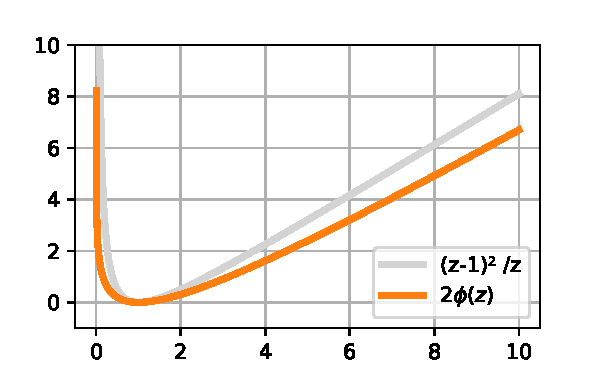
\includegraphics[width=.4\textwidth]{phi.pdf}
	\caption{$\phi(z)$ is the Bregman divergence induced by $-\log(z)$. It is a barrier near $0$. As a result, it is poorly approximated by quadratics, but it admits another upper-bound (in grey).}
	\label{fig:phi}
\end{figure}

\begin{figure}[ht]
	\centering
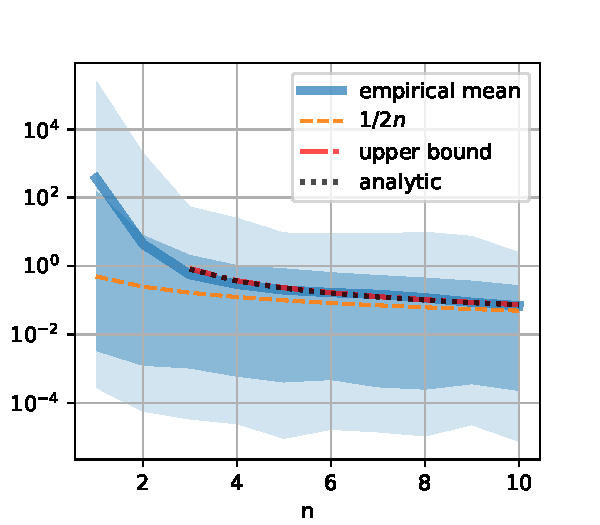
\includegraphics[width=.4\textwidth]{fewsamples.pdf}
	\caption{Suboptimality of a Gaussian variance MLE against number of samples $n$. Bold curve is average over 100 trials,  dark shaded area is 90\% (dark) confidence interval, light shade is min-max interval. 
		While the expected value is infinite for $n=1$ or $n=2$, it quickly matches the upper bound, and the $1/2n$ asymptote.
	}
	\label{fig:curves}
\end{figure}


\begin{theorem}[MLE Tight Bound]
	The MLE of $\cN(0,\m_*)$ is $\hat \m_n^\text{MLE} = \inv{n} \sum_i X_i^2 $.
	Its expected suboptimality is infinite when $n\leq 2$, and otherwise upper-bounded as
	\begin{align}
		 \expect{\bregmanconj( \m_*; \hat \m_n^\text{MLE}) }
			\leq \inv{2n} +\frac{2}{n(n-2)} \; .
			\label{eq:MLE_rate}
	\end{align}
\end{theorem}

This upper bound is asymptotically tight.
We illustrate its numerical behavior in Figure~\ref{fig:curves}.
We get a similar bound for the multivariate generalization :
the expected value is infinite whenever $n \leq d+1$ where $d$ is the dimension, and is otherwise bounded by $O(\frac{d^2}{n} + \frac{d^3}{n(n-d-1)} )$.
  
For the MAP, we get an upper bound thanks to the inequality $ - \log(z) \leq \inv{z} - 1$ which implies
\begin{align}
	\label{eq:log_bound} 
	\phi(z) \leq \half (z + \inv{z}) - 1 = \frac{(z-1)^2}{2 z} \; .
\end{align}

\begin{theorem}[MAP Bound]
 For $n\in \naturalnumbers$, let us  define
 \begin{align}
	b_n = \frac{(1 + \inv{n_0} - \frac{\m_0}{\m^*})^2}{2 (\frac{\m_0}{\m^*}+\frac{(n-2)_+}{n_0})(1 + \frac{n}{n_0} )} \; .
 \end{align}
The expected suboptimality of the MAP of $\cN(0,\m^*)$ with prior hyper-parameters $(n_0,\m_0)$ is
 \begin{equation}
	\expect{\bregmanconj( \m_*; \hat \m_n^\text{MAP})}
	\leq \begin{cases}
		\inv{2(n_0+1)}  +  b_1 \ \text{if}\ n=1,\\
		\frac{1}{n_0 \frac{\m_0}{\m^*} +n-2} + b_n \ \text{if}\ n\geq 2
	\end{cases}
	\label{eq:MAP_rate}
\end{equation}
\end{theorem}

This inequality highlights a clear variance-bias decomposition.
In particular, there is no bias term when $\frac{\m_0}{\m^*} =1 + \inv{n_0} $, which happens when the prior is slightly larger than the ground truth.  For instance, when $n_0=1$, it encourages us to set $\m_0 = 2 \m^*$.
Remark that the variance term is not asymptotically tight as the log-inequality we used \eqref{eq:log_bound} is not quadratically tight around $1$. We are basically losing a factor 2 compared to $1/2n$.


\begin{figure*}[t]
	\centering
	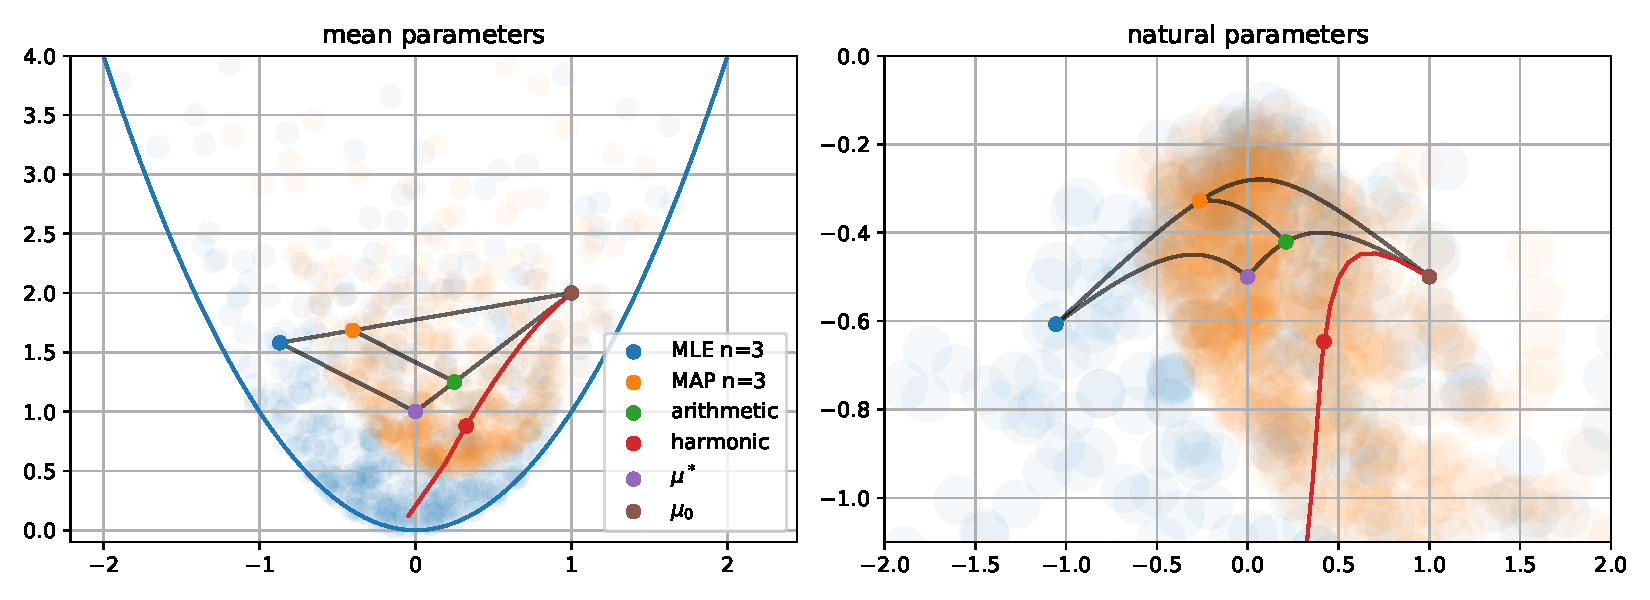
\includegraphics[width=\textwidth]{figs/thales/numerical_schema_n=3.pdf}
	\caption{A numerical illustration of the different characters featured in the bias-variance decomposition, for a 1D Gaussian $\cN(\mu, \sigma^2)$.}
	\label{fig:bias-variance-numerical}
\end{figure*}


\section{Optimization Perspective}
\label{sec:optimization}
As we saw in Section~\ref{ssec:MAP=SMD}, MAP can be interpreted as Stochastic Mirror Descent (SMD). 
There are two consequences of this observation: 1. we may obtain a convergence rate for MAP from an optimization analysis, and 2. any insights gained from the MAP may inform further design and analysis of SMD.

\subsection{Relative Smoothness}
Mirror Descent (MD) \footnote{Mirror Descent is going by many names : Bregman (proximal) Gradient, Relative Gradient Descent, NoLips.} \citep{nemirovski1983problem, beck2003mirror} was first introduced to optimize non-smooth functions, typically under bounded gradient assumption on the objective $f$ or strong convexity assumption on the potential $\logpart$\citep{bubeck}\TODO{bubeck online learning 2011, or monograph?}.

More recently, advances in optimization that go beyond the Euclidean case, 
to optimize a function $f$ when it is not smooth, meaning its gradient is not $L$-Lipschitz,
neither strongly convex in the Euclidean norm, using the concept of relative smoothness 
\citep{birnbaum2011distributed, bauschke2017descent, lu2018relatively}.
Instead of measuring strong-convexity and smoothness in the Euclidean norm (or any norm), 
the $\mu$-strong convexity and $L$-smoothness of a function $f$ 
relative to a reference function $A$ is defined  as 
\aligns{
	\mu \cB_{A}(x, y)
	\leq 
	\cB_f(x,y)
	\leq 
	L \cB_A(x,y).
}
Those conditions ensure the linear convergence rate of mirror descent with $A$ as the reference function.
 Exponential families log-likelihood perfectly fits into this theory.
\aligns{
	f(\theta) = A(\theta) - \expect[x\sim p(x\cond\theta)]{\lin{x, \theta}}
}
is $1$-smooth and $1$-strongly convex relative to $A$.
However, the MAP is stochastic, and known results for stochastic mirror descent do not give convergence rates 
for all exponential families.

{\bf Traditional results}
in stochastic optimization,
such as the work of \citet{nemirovski2009robust,ghadimi2012optimal},
rely on the assumption that the reference function $A$ 
is itself strongly convex relative to a norm $\norm{\cdot}$,
(meaning that $f$ is strongly convex). 
This apply for the MLE problem of a Gaussian distribution 
with fixed variance, 
but not when the covariance is unknown,
or for a Poisson distribution, as $-\log(\theta)$ and $\exp(\theta)$
are not strongly convex.
Relative smoothness has renewed interest for analyses of mirror descent
without relying on strong-convexity in an underlying norm.
However, they do not yet address the problem satisfactorily.

\TODO{table of results of all 3 papers.}

\textbf{An adaptation of the bounded variance,}
investigated by \citet{hanzely2018fastest}, 
defines the following bounded quantity.
Letting $\theta^+(v)$ be a step from $\theta$ with vector $v$, 
$\theta^+(v) = \nabla A^*(\nabla A(\theta) - v)$,
\alignn{\label{eq:assumption-hanzely}
	\expect[\tilde g]{
	\lin{
		\nabla f(\theta) - \tilde g, 
		\theta^+\!\!\paren{\eta \tilde g } - \theta^+\!\!\paren{\eta \nabla f(\theta)}
	}
	}
	\leq 
	\eta C,
}
for some step-size $\eta$ and constant $C$. Let us unpack this quantity; 

{\bf For a Gaussian} with known variance, 
with $A(\theta) = \frac{1}{2}\norm{\theta}^2$, 
this definition recovers the variance of the stochastic gradient
$\expect[\tilde g_t\!\!]{\norm{\nabla f(\theta_t) - \tilde g_t}{}^2}\leq C$.
More generally, if $A$ is $\mu$-strongly convex in $\norm{\cdot}$,
the left-hand side of \cref{eq:assumption-hanzely} is bounded by 
\aligns{
	\frac{1}{\mu} \expect{\norm{\nabla f(\theta_t) - \tilde g_t}{}^2_*},
}
and a uniform bound $C$ exist if the variance of the stochastic gradient is bounded.

{\bf In divergence,} this condition states that the (symmetrized) divergence between 
a deterministic and stochastic update is bounded in expectation,
\aligns{
	&
	\mathbb{E}_{\tilde g_t}\bigg[
	\cB_{A^*}\paren{\mu - \eta g, \mu - \eta \nabla f(\theta)}
	\\
	&\hphantom{\mathbb{E}_{\tilde g}[}
	+ \cB_{A^*}\paren{\mu - \eta \nabla f(\theta), \mu - \eta g}
	\bigg]
	\leq 
	\eta C.
}

{\bf For a maximum likelihood problem, }
where $\tilde g = \mu - x$ 
where $x \sim p(x\cond\theta_*)$,
and $\nabla f(\theta) = \mu - \mu_*$,
\aligns{
	&
	\mathbb{E}_{x}\bigg[
	\cB_{A^*}\paren{(1-\eta) \mu + \eta x, (1-\eta)\mu + \eta \mu_*}
	\\
	&\hphantom{\mathbb{E}_{\tilde g_t}[}
	\cB_{A^*}\paren{(1-\eta)\mu + \eta \mu_*, (1-\eta) \mu + \eta x}
	\bigg]
	\leq 
	\eta C.
}

\fdk{Example where this fails?}

\textbf{Bounded variance at the minimum, }
\fdk{\citep{dragomir2021fast}}

\textbf{Bounded optimality gap,}
\fdk{
Adaptation of the $\expect{\min_x f(x) - \min_x f_i(x)} \leq \sigma^2$ hypothesis \citep{dorazio2021stochastic}}








\bibliographystyle{apalike}
\bibliography{references.bib}


\clearpage
\section{Group Meeting}
\begin{enumerate}
	\item new plots : mirror map, and gaussian trajectories. Add trajectories to paper, with background level set, and new legend : primal/dual expectation
	\item the MLE is biased according to our definition. See plots. Does this definition of bias make sense ? An unbiased estimator's primal mean would be equal to the optimum, vs the dual mean.  Remark : the MLE is biased for standard parameters.
	\item exciting pap er\citet{kakade2010learning}
	\begin{enumerate}
		\item assumption in the spirit of infinite order self-concordance only at the optimum
		\item After a burn-in phase, the loss behaves quadratically. No precise description of the burn-in length.
		\item \TODO{it is worth writing down until the end what we are obtaining with self-concordance.}
		\item idea 1 : try to express some of their results with the mean parameter instead.
		\item idea 2 : using their assumption on the mirror map, perform a Newton kind of analysis for SMD. (exploiting the link MAP -> optimization). How do we prove the linear convergence of Newton to the quadratic regime ? That is the problem at stake here.
	\end{enumerate}
	\item Intro : positioning between optimization and statistics. Start with stats. Convince the reader that this is an essential problem, with asymptotic rate. but finite is elusive. Inspired by recent work (lepriol2021 , bach2013) we want to use optimization to give a rate. We fail, but we reveal a hole in current analysis.  Finite rate would allow us to quantify the importance of the prior, and also help us understand behavior for small numbers. 
	\item Intro : 1 clear question and sharper contributions, with references to sections, as a memo for the reviewer writing his review. "investigate bias-variance..." "we show all these analysis suffer from this problem."
	\item Organization : add optim parallel in insigths section, and then sprinkle references until the optim section.
	\item Optim : find members of the exponential family where the rate of Dragomir et al. holds.
	\item Technical Background : be precise and add reference for the steep exponential family of Legendre type which guarantees that our sets are open, and have a solution in the middle.
	References: \begin{itemize}
		\item \href{https://www.jstor.org/stable/4616462?seq=1#metadata_info_tab_contents}{Existence of Maximum Likelihood Estimates for Multi-Dimensional Exponential Families}, 
		\item The singly truncated normal distribution: A non-steep exponential family, 
		\item Statistical exponential families: A digest with flash cards,
		\item Information and Exponential Families In Statistical Theory, 
		\item Fundamentals of Statistical Exponential Families with Applications in Statistical Decision Theory.
	\end{itemize}  
\end{enumerate}




\section{Blurbs/ideas?}



\subsection{SGD blurb}
\fdk{
%
There is a long line work bounding the convergence rate of stochastic gradient descent.
Beyond the results of \citet{robbins1951stochastic}, 
we now have proofs on smooth, strongly convex problems and bounded variance 
(as well as other assumptions on the noise, reviewed later)
a decreasing step-size and an averaging scheme gets 
a $1/t$ convergence rate, 
which matches the asymptotic rate of unbiased estimation,
through clever averaging schemes \citep{rakhlin2012making,lacostejulien2012simpler} 
\\
Those papers assume the stochastic gradients are bounded, 
but small modifications also work for bounded variance instead.
\\
We do have extensions to other notions of bounded variance, 
for example assuming that the stochastic gradients are gradients of a perturbed smooth function $f_i$ 
and that the minimum of $f$ and the minima of the $f_i$ 
are bounded, $\expect{\min_x f(x) - \min_x f_i(x)} \leq \sigma^2$,
or that the gradient noise is bounded only at the minimum. 
For a review, see \citet{gower2019sgd}.
\\
However, for some problems, combining decreasing step-sizes and averaging is not necessary,
even when the function is not strongly convex.
This is the case for maximum likelihood estimation and matches the asymptotic rates, 
but holds more generally, for example for linear and logistic regressions \citep{bach2013nonstronglyconvex,moulines2011non}.
}


\subsection{Poisson likelihood?}
\fdk{
\citet{bauschke2017descent} and \citet{hanzely2018fastest} both use the example of Poisson inverse problems/Poisson regression
as examples. 
The simpler case of the MLE of a Poisson distribution is also unsolved, though. 
In this case, $h(x) = 1/x!$, $x \in \mathbb{N}$, $A(\theta) = e^\theta$ over $\theta \in \mathbb{R}$,
$A^*(\m) = \m \log \m - \m$ over $\m \in \mathbb{R}_+$.
It is neither strongly-convex nor self-concordant (at least according to the standard definition, 
although it satisfies generalized notions of self-concordance as $A'''(\theta) = A''(\theta)$).
}

\subsection{``simple'' open problem?}
\fdk{
A ``simple open problem'';
assume we have a deterministic problem, so that we know where the minimum is. 
Can we figure out a (deterministic) path from $\theta_0$ to $\theta_*$ 
that has optimality decreasing as $1/n^2$, 
to mirror the bias term of gradient descent?
}

\subsection{Connection with acceleration?}
\fdk{
The problems on how to deal with Bregman divergences abound in optimization, beyond stochasticity. 
For example, we haven't yet figured out the analog of Nesterov-type acceleration 
on relatively smooth and strongly convex problems, 
to bring the convergence rate from linear in $(1-\kappa)$ to $(1-\sqrt{\kappa})$, 
or just from $1/T$ to $1/T^2$ in the (non-strongly) convex case.
\citet{dragomir2021optimal}  shows that naïve application of Bregman updates can not achieve acceleration.
The tools developed to make progress on one problem might help make progress on the other. 
}


\end{document}